\documentclass[tikz,border=2pt]{standalone}
\usepackage{amsmath}
\usetikzlibrary{arrows.meta}
\begin{document}
% Two-stage game (delta = 1, stages t = 0, 1) from the example: play (C,C) at t = 0; after the observed history
% h^1 = (C,C) play the good stage equilibrium (P,P), after any other history the bad one (D,D).
% Player 1 conforming: 4 + 3 = 7; best deviation D at t = 0: 5 + 1 = 6.
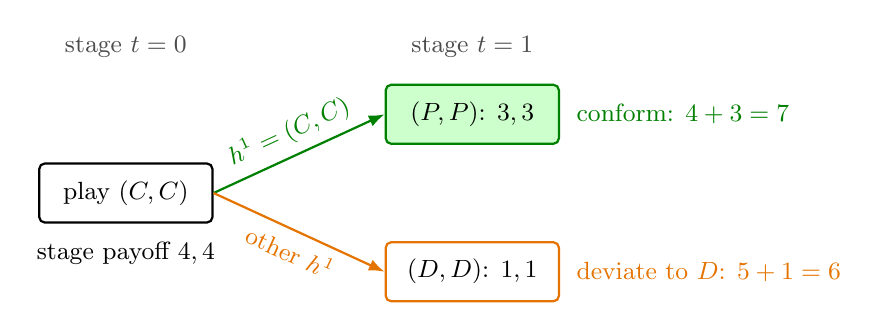
\begin{tikzpicture}[font=\small, >={Latex[length=2mm]},
    box/.style={draw, thick, rounded corners=2pt, minimum width=2.2cm, minimum height=0.75cm, align=center}]
  \node[gray!60!black] at (0,1.85) {stage $t=0$};
  \node[gray!60!black] at (4.4,1.85) {stage $t=1$};
  \node[box] (s1) at (0,0) {play $(C,C)$};
  \node[box, draw=green!50!black, fill=green!20] (g) at (4.4,1) {$(P,P)$: $3,3$};
  \node[box, draw=orange!90!black] (b) at (4.4,-1) {$(D,D)$: $1,1$};
  \draw[->, thick, green!50!black] (s1.east) -- node[above, sloped] {$h^1=(C,C)$} (g.west);
  \draw[->, thick, orange!90!black] (s1.east) -- node[below, sloped] {other $h^1$} (b.west);
  \node[anchor=north, align=center] at (0,-0.5) {stage payoff $4,4$};
  \node[green!50!black, anchor=west] at (5.6,1) {conform: $4+3=7$};
  \node[orange!90!black, anchor=west] at (5.6,-1) {deviate to $D$: $5+1=6$};
\end{tikzpicture}
\end{document}
